\chapter{基于图模型的整体文本分类算法}
由前两章介绍可以得知,文本数据由多个单词构成,每个单词可以视作单一的个体,单词之间又充满着联系,因此
采用图模型建模文本数据,有利于分析单词之间的关联,进而有助于提升模型对文本结构、文本内容的理解,从而提升
模型分析文本,理解数据的能力。因此,本章提出一个基于图模型理论的方法,将文本数据构建为图结构,从单词之间关联
分析文本内容,实现文本分类任务,提升文本分类准确率。
\section{引言}
近年来,图神经网络被广泛应用于学习图的局部和全局的丰富结构信息\citing{wu2019,zhou2018graph},它引起了众多研究者的极大关注。
文本数据并不是一种天然的图结构数据,因此需要人为的定义规则去构建图。Yao等人\citing{yao2019graph}就提出了一种基于图模型的文本
分类算法。他们首先根据语料库中词的共现信息以及文档与单词之间共现关系为边,构建了一个使用单词作为节点以及文档也作为节点的图。
然后采用GCN学习单词以及文档节点的向量表示。该方法在测试数据集上展现了良好的分类性能。但是这个方法忽略了单词在句子中的顺序,同时由于
整个语料库中单词表示仅有一个,忽略了单词在不同语境下可能具有不同的含义,最重要的一点即是构成的图是依据整个语料库构建的单一图,结构
是固定不可更改的,因而图的大小取决于语料库的大小,语料库过大将会导致图模型难以计算,同时更难以扩展到新的文本数据中。

本章提出一个基于图卷积神经网络(GCN)的文本分类算法。具体来说,该算法为语料库中的每个文本构建一个图,不同于Yao\citing{yao2019graph}的
方法,仅使用单词作为节点,而不考虑文档作为节点。这样有助于捕获词之间在空间、时间和上下文中的信息。
同时算法还为每个图创建一个连接到所有单词节点的“虚拟”超节点,它专门用作上下文感知组件,用于学习文档全局的特定信息。
经过GCN学习后,获得了单词新的向量表示以及一个超结点的向量表示。超结点的向量表示可以视作为文本数据全局信息表示。而对于新的单词向量表示,将其
输入到一个卷积神经网络网络(CNN)用以学习文本数据中局部信息以及序列信息。最终,算法融合超结点向量信息以及CNN模型学到的向量信息,作为
最终的文本向量表示,用以文本分类任务。

综上所述,本研究的主要特点有两个方面。\noindent\textcircled{1}本章提出了一种基于图模型的文本分类方法,通过单词之间的
关系构建图,通过图模型学习,从而进一步优化单词向量表示。\noindent\textcircled{2} 构建超结点学习文本的全局信息,结合CNN提取出的局部信息
,相比于目前较为常用的方法,模型分类准确率有一定提升。本章第二节对整体文本分类任务问题进行阐述,第三节介绍算法的整体设计,第四、五节
则对模型采用常用的数据集进行验证。

\section{问题定义}
本章主要研究的是对文本数据进行分类的算法。比如一个文本“a very funny movie”,纵观整个句子,从“funny”这个词就能分析出
这句话的情感是正向的,因此整个文本即可归为正向分类。整体文本分类算法是从具体整体含义出发,确定文本所属的某一
类别。

某一文本数据$T_i$由一组$n$个单词构成,$T_i=[w_1,w_2,...,w_{n-1},w_n]$,其中每个单词$w_i$都会有一个初始化的向量$v_i$,
向量可以是随机初始化,也可由各类单词向量表示学习方法获得。因此一个文本可以由一个$\mathbb{R}^{n\times d}$的向量矩阵表示,其中$n$
表示文本中单词的个数,$d$表示为单词向量的维度。文本分类任务就是学得一个函数$F(\cdot)$,通过输入一个文本数据,然后得出该文本所属的类别
,通过一个文本仅对应一个类别。比如根据一段新闻的描述,判断它是属于财经类新闻,还是娱乐明星类的新闻。


\section{算法模型设计}
传统的文本分类算法忽略文本在语料库中整体的统计信息,以及单词之间的互相影响。
因为单词之间互有关联,尤其是同一个句子中的单词含义应该与整个句子的语义有关,而通常的单词嵌入模型每个词向量仅有一种。
因此本章算法采用图模型将单词之间的信息通过图网络互相传递,重新学得更符合整个句子语义的单词的表示。
同时还结合每个单词在整个语料库的统计信息,进一步生成代表整个文本含义的特征向量表示。
对于单词向量继续采用常规的CNN模型进行分析,再与单词统计信息学的到特征向量相结合,最终实现文本分类任务。
本节主要详细介绍算法模型,命名为TextGraph。首先介绍了模型的整体设计,随后详细介绍每一步的具体实现及算法细节。
\subsection{模型总览}
\begin{figure}[htb]%\small tbp
	\setlength{\belowcaptionskip}{0pt}
	\centering
	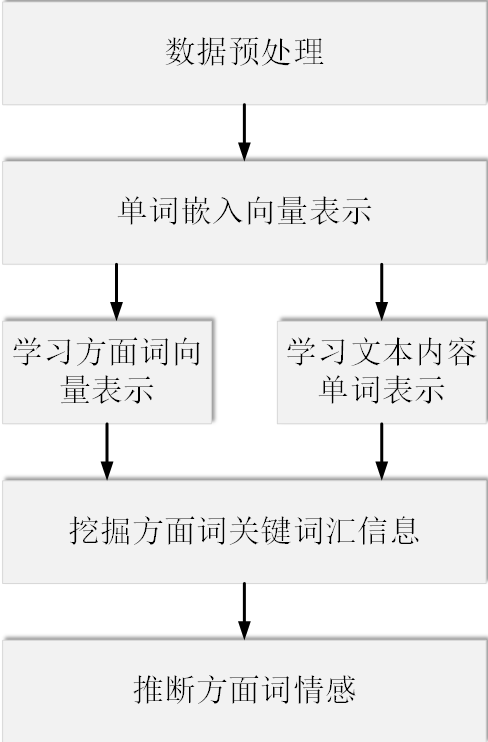
\includegraphics[width=0.3\textwidth]{pic/textgraphLct.png}
	\caption{文本分类算法计算过程}
	\label{textgraphLct}
\end{figure}

本章实现的文本分类算法计算过程如图\ref{textgraphLct}所示。数据预处理主要是指自然语言处理前需要对文本数据进行统一的规则化处理,
比如将所有文本都处理成小写字体,同时删除部分无关的词汇,如一些停止词等。
此外还需要建立词汇表,其中不同的单词应该对应一个唯一的索引,有助于后期处理时正确找到每个单词所对应的嵌入向量。
\begin{figure}[htb]%\small tbp
	\setlength{\belowcaptionskip}{0pt}
	\centering
	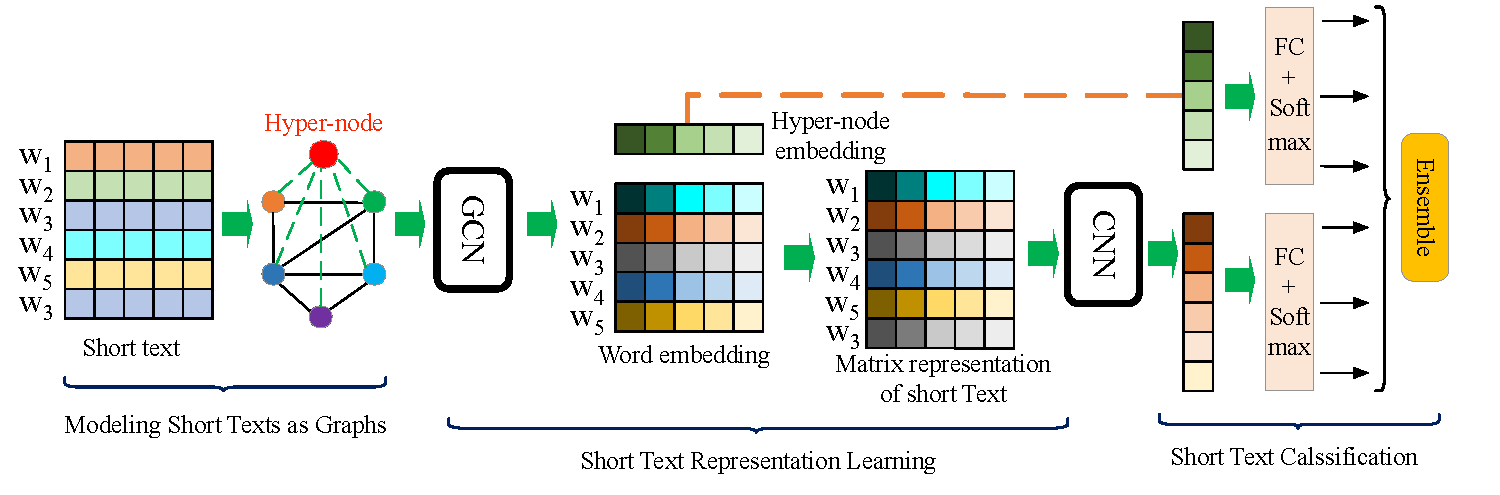
\includegraphics[width=1\textwidth]{pic/TextGraph-arch.pdf}
	\caption{TextGraph模型}
	\label{TextGraph}
\end{figure}

TextGraph是一个端到端的模型深度学习模型,输入文本数据,输出文本的标签分类。该算法共有三个部分,如图\ref{TextGraph}所示,
第一部分定义为文本构图,即通过一些方法,将文本数据转化为图结构,转化为后面算法计算需要的数据。
第二部分为单词向量表示学习以及CNN网络对文本特征提取,即采用图模型对构成的文本结构图进行学习,获取新的单词向量表示。
对新的向量表示再采用CNN网络提出文本的特征,主要是局部特征。
第三部分为向量信息融合及分类,通过前两步学习,可以获得一个超结点的向量
以及经过CNN池化后的文本向量,两种向量从不同方面学习到了文本的信息,将两类向量进行融合提升模型准确率。以下几节将分别对这些部分
进行详细介绍。
\subsection{文本数据建模为图结构}
TextGraph将文本数据构建为一个带权的有向图,其中每个单词即为图的一个节点,边表示为单词之间的某种联系。同时,该算法创建了一个超节点,
这个节点连接到所有的单词节点,同时采用特殊的计算方式构建与其他单词之间的权重。超结点可以理解为全局信息表示,在模型训练过程中,获取文本的
整体信息,同时将这些信息传递给其他单词节点,使得单词节点信息表示更加丰富。图中节点的初始化属性即为单词的属性,这类属性通常由单词向量表示学习
方法获得,例如GLoVe方法\citing{pennington2014glove},有时也可以采用随机初始化的方式表示单词属性,如高斯分布下的随机初始化。

\begin{figure}[htb]
    \setlength{\belowcaptionskip}{0pt}
    \centering
    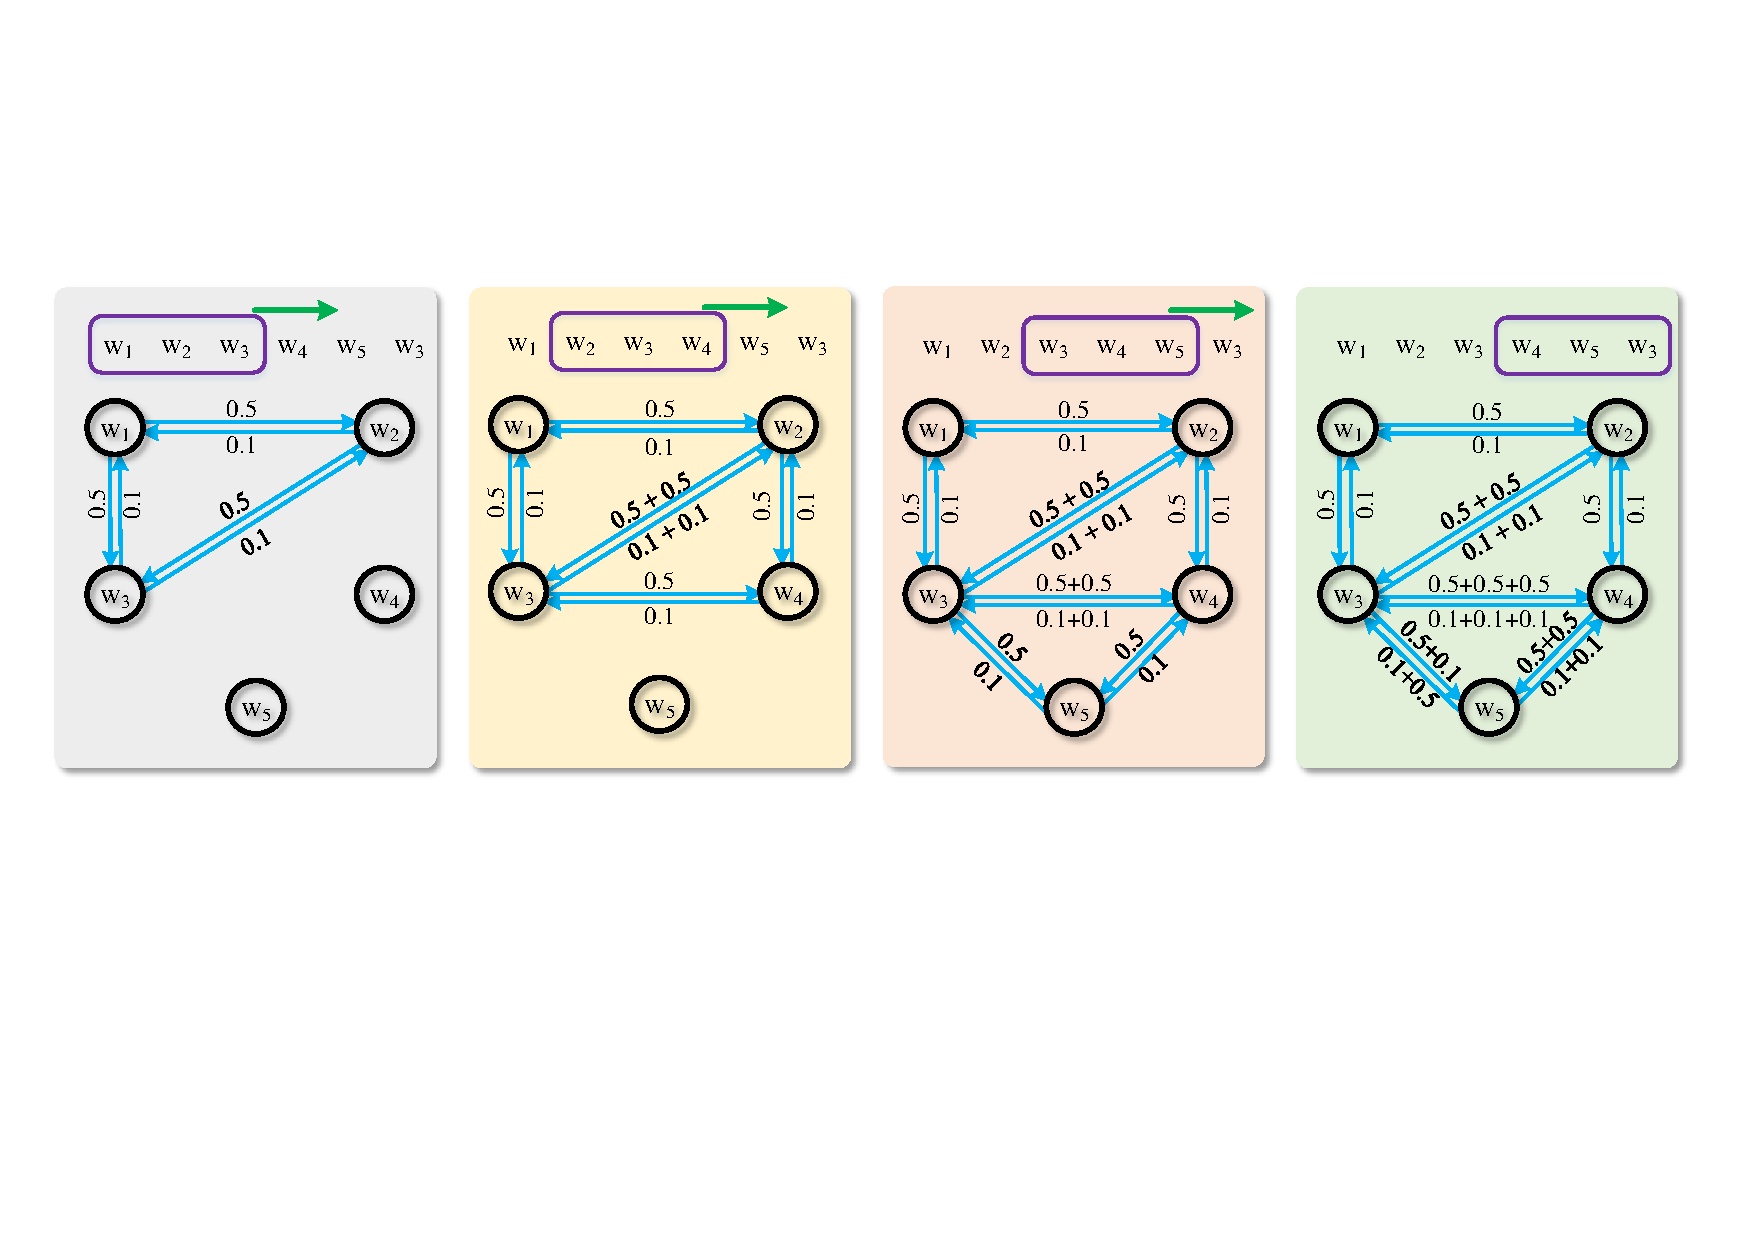
\includegraphics[width=1\textwidth]{pic/text2graph.pdf}
    \caption{图构建过程}
    \label{text2graph}
\end{figure}

为了获得带权重的有向图,该算法采用了滑动窗口策略实现。滑动窗口的大小$m$是固定的,主要根据实验结果获得。该策略详细步骤如下。
滑动窗口是对文本的单词进行滑动,每个窗口内根据窗口大小$m$,包含$m$个单词。在窗口中,单词与单词之间构成一个单词对,前一个单词对于后一个单词具有
权重$w_f$,后一个对于前一个单词具有权重$w_b$,其中$w_f$和$w_b$也是预先定义的固定大小的值,为了反映序列信息,通常这两个值不一样。
因此滑动窗口大小$m$和权重$w_f$和$w_b$是可调节的超参数。滑动窗口依次从左向右移动一个单词距离。如果已经存在连接两个单词的边,则将累积相应的权重。
这个过程不断迭代,直到滑动窗口覆盖了文本的最后一个单词。如图\ref{text2graph}所示,给定的文本序列是$[w_1,w_2,w_3,w_4,w_5,w_3]$,其中每个$w_i$是一个单词。
为了简单起见,将参数设置为$m=3$、$w_f=0.5$和$w_b=0.1$。开始时,滑动窗口覆盖$[w_1,w_2,w_3]$这三个单词,因此构成了
前向边$(w_1,w_2)$,$(w_1,w_3)$,和$(w_2,w_3)$,每个权重均为0.5。同时,后向边有$(w_2,w_1)$,$(w_3,w_1)$,和$(w_3,w_2)$,其权重为0.1。
然后,滑动窗口向右移动一个单词,到达$[w_2,w_3,w_4]$这个序列。由于边$(w_2,w_3)$已经存在,新的权重将变为$0.5+0.5$。
同样,对于边$(w_3,w_2)$,新的权重变为$0.1+0.1$。此过程一直持续到最后一个窗口$[w_4,w_5,w_3]$。单词$i$和单词$j$之间的累计权重由$a_{ij}$表示,
该算法通过滑动窗口的总数来规范化$a_{ij}$,计算方式为$\frac{a_{ij}}{c}$,其中$c$为滑动窗口次数。超结点则是连接到所有其他单词节点的一个虚拟节点,其
边的权重由整个语料库中单词的TF-IDF计算得到。因此节点与节点之间的权重$A_{ij}$可以由公式\ref{weightGraph}得到。
\begin{equation}\label{weightGraph}
A_{ij}=
\begin{cases}
\frac{a_{ij}}{c}& \text{当 $i, j$ 都是单词时}\\
TF\text{-}IDF(i) & \text{当$i$ 是单词, $j$ 是超结点时}\\
1 & \text{$i=j$}\\
0 & \text{其他情况}
\end{cases}
\end{equation}

因此,对于图\ref{text2graph}中的文本的邻接矩阵$A$可以如下公式\ref{adjacentmatrix}表示,该矩阵不包含超结点的权重信息。
\begin{equation}
    \label{adjacentmatrix}
    A=\left[
    {\begin{array}{*{20}{c}}
     {\text{1}}&{{\text{0}}{\text{.5/4}}}&{{\text{0}}{\text{.5/4}}}&{\text{0}}&{\text{0}} \\
     {{\text{0}}{\text{.1/4}}}&{\text{1}}&{\text{1/4}}&{{\text{0}}{\text{.5/4}}}&{\text{0}} \\
     {{\text{0}}{\text{.1/4}}}&{{\text{0}}{\text{.2/4}}}&{\text{1}}&{{\text{1}}{\text{.5/4}}}&{{\text{0}}{\text{.6/4}}} \\
     {\text{0}}&{{\text{0}}{\text{.1/4}}}&{{\text{0}}{\text{.3/4}}}&{\text{1}}&{\text{1/4}} \\
     {\text{0}}&{\text{0}}&{{\text{0}}{\text{.6/4}}}&{{\text{0}}{\text{.2/4}}}&{\text{1}}
    \end{array}}
    \right]
    \end{equation}

\subsection{表示学习过程}
文本分类效果取决于单词嵌入表示的学习以及文本表示学习过程,TextGraph通过GCN网络重新学习到单词向量表示,
再将学习到的向量表示输入到CNN网络结构中进一步提取特征信息,以达到最优的特征提取。

本章采用GCN网络去学习构建好的文本图数据。通过多层的GCN,单词节点不仅能够获取与自己在同一窗口下的其他单词信息,
也能获取得到得更远的单词信息。单词之间的信息可以通过构建好的边进行共享。而对于超结点,因为包含了语料库中
单词的共现信息——通过TF-IDF方法获得到的,因此超结点在GCN网络学习的过程中,会获得整个文本的全局信息,同时这些信息
也会选择性的传递给所有单词节点,以辅助单词节点学习到更加丰富的表示。同时,采用了注意力机制辅助模型在学习的过程中关注于
重点信息。即有些单词之间虽然具有边,但是由于这些单词之间关联程度并不高,采用注意力机制有助于降低对不重要信息的关注,
将更多注意力放在重点的单词节点上进行信息传递。因此对于单词$i$,$j$之间的注意力分数可以通过公式\ref{TextGraphAttFor}得到。
\begin{equation}\label{TextGraphAttFor}
    \gamma_{ij}=sigmoid(x_iW_{a1})+sigmoid(x_jW_{a2})
\end{equation}

$\gamma_{ij}$即为注意力分数,其中$W_{a1}$和$W_{a2}$为$d\times 1$的权重矩阵,$x_i$,$x_j$为当前单词$i,j$的向量表示,
为$1\times d$的向量。$sigmoid$为激活函数。加入注意力机制后,与形如公式\ref{GNNFormula1}所示的GCN计算方式略
有不同,对于每一层的单词向量表示计算可以由公式\ref{TextGraphLayerFor},\ref{A_hat},\ref{D_hat}计算得到。
\begin{equation}\label{TextGraphLayerFor}
    H^l=\sigma((\gamma ^l\hat{D}^{-\frac{1}{2}}\hat{A}\hat{D}^{-\frac{1}{2}})H^{l-1}W^l)
\end{equation}
\begin{equation}\label{A_hat}
    \hat{A} = A+I
\end{equation}
\begin{equation}\label{D_hat}
    \hat{D} = \sum{j}A_{ij}
\end{equation}
其中$H^l$为$n*d$的矩阵,第$i$行的向量表示为文本序列中第$i$个单词的在GCN网络中第$l$层的向量表示,为一个$1\times d$的向量。
$\gamma ^l$则为第$l$层计算得到的权重矩阵。

经过GCN网络学习后,每一单词向量都得到更新,获得了新的向量表示,假设第$i$个单词的输出向量为$h_i\in \mathbb{R}^k$,其是一个、
$k$维的单词向量。因此对于一个包含$n$个单词的文本序列可以获得一个$H\in \mathbb{R}^{n\times k}$的矩阵,即$H=[h_1, h_2,\cdots, h_n]^T$。

为了得到文本的局部信息以及序列信息,本算法采用一个一维卷积神经网络(CNN)结构提取相关特征。
其中CNN网络中的卷积核$\mathbf{w} \in \mathbb{R}^{h\times k}$是一个$h \times k$的权重矩阵,
$h$表示为当前CNN网络的卷积窗口大小为$h$,即每次窗口考虑$h$个单词用以计算特征值,计算公式如\ref{cnnFor}所示。其中$\sigma$
是一个激活函数,$b$是偏置矩阵。
\begin{equation}\label{cnnFor}
    f_i=\sigma(\mathbf{w} \cdot y_{i:i+h}+b)
\end{equation}

文本数据的卷积操作不同于图像数据,只会在文本序列的一个方向做卷积,即在垂直方向做卷积。卷积核每次移动向下一个单词移动一次,如图\ref{cnnslide}所示,红色线框为卷积核,每次计算
生成一个特征值,之后向下移动一步,如虚线框所示。因此这样的卷积操作下,将会生成$(n-h+1)$个特征值。
\begin{figure}[htb]
    \setlength{\belowcaptionskip}{0pt}
    \centering
    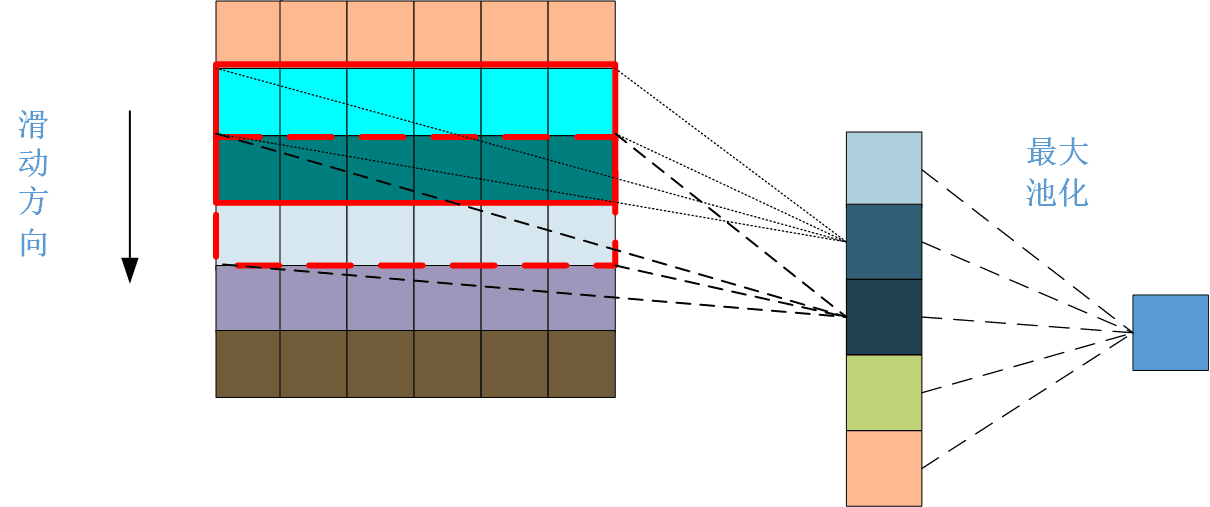
\includegraphics[width=0.6\textwidth]{pic/cnnslide.png}
    \caption{CNN特征生成过程}
    \label{cnnslide}
\end{figure}

对于每一个卷积核都会产生一组特征值,为了获取其中最关键的特征,本算法采用最大池化操作进行特征提取。最大池化操作即是选择这一组
特征中值最大的。
最大池化操作有助于选取最重要的特征,比如一句话“这个公园景色不错,但是我今天玩得并不开心。”,虽然这句话
从前面的信息来看好像是正面的表述,实际上通观全文,最后的“玩得并不开心”的信息才是最重要的。
通过选择每个卷积核中的提取的特征的最大值,可捕获其最重要的特征。这样操作后每一个卷积核得到特征就是一个值。
另一方面,采用池化操作有助于降低参数量,进而可以减少模型过拟合问题。经过多个卷积核的卷积池化操作后,将这些所有卷积核产生
的特征值拼接起来就能得到文本的特性向量表示。

\subsection{向量融合及分类}
经过以上步骤,将获得一个超结点的向量表示$e_h$,这个向量可以理解为对全局信息的捕捉;以及经过CNN网络提取得到的文本向量表示$e_c$,
这个向量可以理解为对局部信息以及重点关注信息的表示。总之,这两个向量都可以作为文本的向量表示,只是包含的信息内容有所不同。
$e_h$和$e_c$都可以单独作为结果实现文本分类。而两者的结合将会获得表示更加充分的文本向量。

本章,采用两个不同的线性变化层,将$e_h$和$e_c$向量转为为与标签大小$m$同一维度,如公式\ref{eh1},\ref{et1}所示:
\begin{equation}\label{eh1}
    s_h=softmax(e_h \cdot \mathbf{w}_{f1}+b_1)
\end{equation}
\begin{equation}\label{et1}
    s_c=softmax(e_c \cdot \mathbf{w}_{f2}+b_2)
\end{equation}

其中$w_{f1}\in \mathbb{R}^{d_1 \times m}$为$d_1\times m$的参数矩阵,$w_{f2}\in \mathbb{R}^{d_2 \times m}$
为$d_2\times m$的参数矩阵.$d_1$、$d_2$分别为$e_h$和$e_t$的维度大小。softmax为激活函数,是将一组数值压缩到0-1之间,它们的和为1,
可以近似的看做是预测概率。对于分类任务而言,一个$1\times m$的输出向量经过softmax计算后,每一位置上的值
可视作这个位置上对应的标签的概率。softmax计算如公式\ref{softmax}所示:
\begin{equation}\label{softmax}
    s=\frac{e^{e_i}}{\sum\limits_{j}{e^{e_j}}}
\end{equation}

其中$e$为自然底数,经过以上公式计算得到了来至于超结点的预测结果$s_h$以及来自CNN的预测结果$s_c$。为了平衡两者预测的影响,本节采用了一个
超参数$\alpha$去控制,如公式\ref{output}所示。$\alpha$ 取值在0-1之间。
\begin{equation}\label{output}
    O=(1-\alpha) \times s_h+\alpha \times s_c
\end{equation}

因此对于整个模型来说代价函数$C$可以由公式\ref{costFun}得出。
\begin{equation}\label{costFun}
    C=-\frac{1}{M}\sum \limits_{x}\left[(1-\alpha)(ylna_h+(1-y)ln(1-a_h)+\alpha(ylna_c+(1-y)ln(1-a_c)\right]
\end{equation}

其中$M$表示为所有样本数,$x$代表一个样本,$y$表示当前这个样本的真实标签,$a_h$表示为超结点向量
最终的预测结果,$a_c$表示为CNN提取的文本向量最后的预测结果。

\section{实验设置}
\subsection{数据集描述及数据处理}
本章使用文本分类任务中广泛使用的一些数据集,其中包括R8、R52、MR、Yelp等数据集。本章分别在这四种数据集上进行验证模型及与其他模型进行对比。

\textbf{R8和R52}数据集是广泛被使用的一种用于文本分类任务的数据集,其主要来至于路透社的新闻数据。因此其为英文文本数据集。
对于R52来说总共有6532个训练集样本以及2568个测试集样本,平均文本长度为69.82,共计52种分类类别。R8数据集共计有5485样本用做训练集,
2189个样本用作测试集,平均文本长度65.72,共计8个不同的类别标签。
以R8数据集为例,其文本数据如“us house speaker wright concerned of interest rate rise under greenspan ”,该文本数据对应的标签为“interest”,即对于R8数据集
来说,是对文本数据打上最符合的8种标签中的一个。

\textbf{MR}\citing{pang2005seeing}数据集是一种在每个文本序列中只包含一种情感的电影评论数据集。它包括5331个负面情感数据样本以及5331个正面情感的样本,其平均长度为20.39。
本章中采用Tang等人\citing{tang2015pte}使用的训练集测试集划分方式。
MR数据集中数据如“the cast is phenomenal , especially the women”所示,其中这个文本对应的标签为“1”,即代表为正面情感。MR总共两种情感,数据集中分别
用“0”,“1”分别表示负面情感和正面情感。

\textbf{Yelp}也是一种评论数据集,其标签是1-5之间的分数,共计5种标签。为了平衡数据集划分以及控制文本数据集的长度,
本章对这类数据集中的所有数据进行随机抽取,仅抽取文本长度在150个以下的,最终共计获得18972个数据集样本,其中包含14000个用作训练集,4972个用作测试集,
同时将平均文本长度在81.17。
取其中一个文本为例,Yelp数据集文本如“awesome mall all kinds of stores we dont have on the west side ! !”,这段文本对应的标签为“4”,即对于Yelp数据集来说,
每个文本都有一个在1-5之间的标签。

以上四种数据集详细统计如表\ref{summary}所示。

\begin{table*}[htb]
	\centering
	\caption{数据集数据统计}
	\setlength{\tabcolsep}{2mm}{
		\begin{tabular}{c|c|c|c|c|c|c}
			\hline 
			{数据集} & {总文本数} & {训练集数}& {测试集数} & {单词数} & {类别数}& {平均长度}  \\
			\hline 
			$ \text{R8} $ & $ 7,674 $ & $ 5,485 $& $ 2,189 $ & $ 7,688 $ & $ 8 $ & $ 65.72 $ \\ \hline
			$ \text{R52} $& $ 9,100 $& $ 6,532 $ & $ 2,568 $ & $ 2,568 $& $ 52 $& $ 69.82 $  \\\hline
            $ \text{MR} $&$ 10,662 $& $ 7,108 $& $ 3,554 $ & $ 18,764 $ &$ 2 $& $ 20.39 $ \\\hline 
            $ \text{Yelp} $&$ 18,972 $& $ 14,000 $& $ 4972 $ & $ 26,889 $ &$ 5 $& $ 81.17 $ \\\hline 
		\end{tabular}%
		\label{summary}%
	}
\end{table*}

本章中使用的均为英文数据集,因此不用考虑像中文分词。由于英文单词有大小写之分,例如希望在文本处理过程中将“No”和“no”
视作是一个词,因此一般需要将所有的词都转化为小写。同时在文本中存在一些停用词,即许多对分类任务没有太大帮助的词语,比如“aha”、“oh”等,
因此也将这些词语去掉。如句子“No one wants to see this movie. Oh, it's too bad” 经过预处理后变为“
no one wants to see this movie. it's too bad”。对自然语言的文本数据,计算机是无法直接理解的,需要将其转化为计算机能够识别的数据。
本章使用GloVe作为词向量初始化输入。首先对于一个句子,采用“空格”作为分割,将一句话转化为单词列表,如上句子转为单词列表即为
\centerline{$[no,one,wants,to,see,this,movie,it's,too,bad]$}

同时根据整个语料库对所有的单词进行一个唯一编号,本章根据单词出现的顺序进行编号,每个单词
均有一个数字作为唯一标识,如上句单词列表经过编号转化后,可能表示如下:

\centerline{$[4,487,3667,34,1,555,676,12465,376,89]$}

每个编号同时还对应着一个维度为300的唯一的向量表示,来自于GloVe。例如单词“no”在GloVe中的向量表示如下:


\centerline{[-0.015103  -0.618705  0.127657  0.020094  0.186504 }

\centerline{...}

\centerline{0.032921  -0.153918  0.827338  -0.409457]}

也即是编号“4”对应的向量如上。例如对于一个单词数量为18764的MR数据集,便有18764个对应的词向量。如果词向量不存在于GloVe
中,则采用随机初始化的方式生成。因此上述句子便能转为一个形如下的向量矩阵:

\centerline{[-0.015103  -0.618705  0.127657  0.020094  0.186504 }

\centerline{...}

\centerline{0.032921  -0.153918  0.827338  -0.409457]}

\centerline{[0.115103  -0.612235  0.432126  0.045531  -0.488512 }

\centerline{...}

\centerline{-0.132921  0.148618  0.395361  0.642315]}

\centerline{...}

\centerline{[0.515103  -0.122212  0.007217  0.123204  -0.076414 }

\centerline{...}

\centerline{0.102212  -0.000123  0.464318  0.100671]}

最后这样的一个单词矩阵就可以作为计算机可以识别的输入。
\subsection{对比方法介绍}
本章提出的方法是用于实现整体文本分类任务,即一个文本对应一个标签类。因此,所对比的方法都是用于该文本分类任务,且均采用
GloVe词向量作为单词的初始化向量。所涉及的比较方法均属于深度学习模型,且是目前广泛使用的自然语言处理模型。比较模型主要包括以下:

\textbf{LSTM:} 是一种特殊的RNN模型,可以解决长序列训练过程中的梯度消失和梯度爆炸问题,相比于普通的RNN模型,具有更优异的表现。
LSTM每一个循环中,对于输入的单词向量均会产生一个隐藏向量表示,本章中将这些生成的单词的隐藏向量表示做一个平均池化作为文本的向量,
用于实现文本分类任务。

\textbf{Bi-LSTM}\citing{schuster1997bidirectional}: 是一种双向的LSTM模型。它将一个句子从前到后进行处理,同时对句子从后到前进行编码,最后将
两种信息拼接起来。相比于LSTM多了一个从后到前的信息,这样的设计有利于模型进行更细粒度的理解,更好的捕捉双向的语义依赖。本章中采用LSTM获取文本
向量的方式,对通过前向LSTM获得到的文本向量以及从后向LSTM获取的到的文本向量进行拼接,作为最终的文本向量表示,以用于分类任务。

\textbf{TextGCN:}TextGCN\citing{yao2019graph}将单词和文档视作图中的节点,通过GCN进行半监督学习单词节点和文档节点的向量表示,这些节点使用one-hot向量进行初始化。
学习到的文档节点表示即可直接用于实现文本分类任务。

\textbf{TextCNN:}本章采用由\citing{kim2014convolutional}提出的CNN处理文本的方法。对比实验采用一维卷积,对于卷积后的特征值采用最大池化的方式
挑选最重要的特征值。多个卷积核生成多个卷积池化后的特征,将这些特征拼接作为文本向量表示,实现文本分类任务。

\textbf{RCNN:}Lai\citing{lai2015recurrent}等人提出一种将循环神经网络与卷积神经网络中的特点相结合的方法。它首先通过RNN网络获取文本信息,然后采用CNN中的
池化操作提取这些信息中的重要部分。最终获得表示文本的向量,用以实现文本分类任务。

\textbf{MLP:}作为最基本的神经网络对比方法,本章中将一个文本中的所有词向量进行拼接,然后将获得的向量输入一个仅包含输入层、隐藏层和输出层的神经网络实现文本分类任务。

\textbf{HAN:}Hierarchical Attention Networks\citing{yang2016hierarchical}是一种结合了双向RNN和注意力机制的神经网络模型。这个模型关注单词之间的关系,同时也关注句子段与句子段的关系。
即它将一个句子分为多段,在每一段中首先将单词输入双向RNN网络中获得每个单词的隐藏向量表示,之后采用注意力机制将这些单词向量进行加权和获得当前句子段的向量表示。对每一个句子段均采用
这种方式学习向量表示。多个句子段获得多个向量表示,再采用双向RNN网络学习这些向量的新的向量表示,最后将这些学到的句子段向量表示使用注意力机制结合成一个单一的向量,用以表示文本的向量,用作文本分类任务。

\textbf{TextGraph-CNN:}本章提出的方法主要结合了超结点的向量以及CNN提取的向量,因作为对比验证,仅使用CNN提取后的特征向量作为最终的文本向量表示,用以分类,不再结合超结点的向量。

\textbf{TextGraph-HN:}与TextGraph-CNN类似,作为对比,仅使用超结点向量作为文本向量表示。
\subsection{模型训练及验证}
对于所有的对比方法以及本章提出的方法均使用来自于GLoVe的300维预训练单词向量作为初始化,同时均采用相同预处理方式得到的文本数据集。
均采用Adam\citing{2014Adam}优化器对模型进行训练更新权重,且所有模型的学习率都设置为0.001。所有模型都采用相同的超参数,即使用相同大小的隐藏层神经元,本章中均设置为128。对于HAN网络,
本章中设置将一个句子划分为3段。对于TextGraph模型,本章将单词建模过程中的窗口大小设置为4,GCN网络层数为2,采用的CNN网络中的卷积核大小与对比方法TextCNN中采用的
卷积核一致,均使用3,4,5大小的卷积核,同时每种大小的卷积核都有128个。所有模型训练中都采用dropout\citing{2014Dropout}值为0.5防止网络训练过程中的过拟合问题。

为了测试模型之间的性能,所有数据集均划分为训练集和测试集,模型在训练集上进行训练,在测试集上进行验证。

为了验证模型对于随机初始化向量的学习能力,即在不依赖预训练单词向量的前提下,是否依然具有良好的分类性能。实验中不采用GloVe方法中获取得到预训练向量,而是采用
高斯分布随机生成300维的向量用做单词向量的初始化。所有模型在训练集中通过反向传播更新单词向量表示,测试时直接采用训练过程中学到的单词向量表示作为输入进行验证。

为验证模型在少量训练集的情况下的学习能力,本章中采用挑选R8数据集中的部分训练集数据作为模型训练的数据。挑选比例分别设置为2.5\%,5\%,7.5\%,10\%,12.5\%,即训练样本数
分别为137,274,411,548,685,其余所有的数据集则作为测试集验证模型的分类性能指标。

模型分类性能影响可能来至于学习到的向量表示之间是否有较为分明的界限,因此本章中挑选R8数据集文本向量学习结果,采用2维的t-SNE方法实现可视化。本章对比了LSTM模型和TextGraph之间的
可视化差异。
\subsection{实验评价指标}
因为文本分类主要是多分类任务,本章中主要采用准确率(accuracy)和macro-F1分数来验证模型的分类性能。
对于了解这些评价指标首先得了解TP(True Positive )、TN(True Negative)、FP(False Positive)、FN(False Negative)。

\textbf{TP:}即真实的正样本。

\textbf{TN:}即真实的负样本。

\textbf{FP:}即假的的正样本。

\textbf{FN:}即假的的负样本。

因此对于二分类的准确率(accuracy)计算如公式\ref{acc}所示。
\begin{equation}\label{acc}
    accuracy=\frac{TP+TN}{TP+TN+FP+FN}
\end{equation}

由于本章涉及的均为多分类,因此准确率(accuracy)计算方式可以归纳为如公式\ref{accM}所示,$T$表示为所有预测正确的样本数,$F$表示为所有预测错误的样本数。
\begin{equation}\label{accM}
    accuracy=\frac{T}{T+F}
\end{equation}

另外精确率(Precision)P和召回率(Recall)R的计算方式分别为公式\ref{PRE}、公式\ref{RECALL}所示。
\begin{equation}\label{PRE}
    Precision=\frac{TP}{TP+FP}
\end{equation}
\begin{equation}\label{RECALL}
    Recall=\frac{TP}{TP+TN}
\end{equation}
而计算macro-F1分数需要由macro-Precision和macro-Recall得到,计算方式如公式\ref{mPRE}、公式\ref{mrec}、公式\ref{mf1}所示,
其中$P_i$,$R_i$分别表示标签$i$的精确率和召回率。
\begin{equation}\label{mPRE}
    macro-Precision=\frac{1}{D}\sum_{i}{P_i}
\end{equation}
\begin{equation}\label{mrec}
    macro-Recall=\frac{1}{D}\sum_{i}{R_i}
\end{equation}

\begin{equation}\label{mf1}
    macro-F1=\frac{2*macro-Precision * macro-Recall}{macro-Precision + macro-Recall}
\end{equation}

本章设置的对比实验中均采用准确率(以下简称ACC)和macro-F1分数(以下简称F1-score)这两个指标来进行展示与分析。
\section{实验结果及分析}
\subsection{模型分类性能分析}
本小节主要比较了采用GloVe预训练的词向量初始化以及采用随机初始化的模型之间的差异。

如表\ref{tab:acc-result}所示,展示了采用GloVe预训练的模型的准确率(ACC)和F1分数(F1-score),可以明显看出本章提出的
模型在所有数据集上均取得了最优的分类结果。

\begin{table*}[htb]
    \centering
    \caption{ 采用预训练词向量下的各模型分类性能比较}
    \renewcommand\arraystretch{1}
    \renewcommand\tabcolsep{2mm}
    \label{tab:acc-result}
    \arrayrulecolor{black}
    \begin{tabular}{lcccccccc}
    \hline
    \multirow{2}{*}{\textbf{Models}} & \multicolumn{2}{c}{\textbf{MR}} & \multicolumn{2}{c}{\textbf{R52}} & \multicolumn{2}{c}{\textbf{R8}} & \multicolumn{2}{c}{\textbf{Yelp}}  \\
    \cline{2-9}
                            & ACC   & F1-score       & ACC   & F1-score        & ACC   & F1-score       & ACC   & F1-score          \\
    \hline
    TextGCN                 & 76.74 & 76.72         & 93.56 & 65.51          & 97.07 & 92.41         & -     & -                 \\
    TextCNN                 & 78.16 & 78.16         & 93.90  & 67.37          & 97.24 & 92.57         & 51.52 & 45.15            \\
    HAN                     & 77.78 & 77.67         & \underline{94.64} & \underline{74.62}          & 97.15 & 93.62         & 53.51 & 48.91            \\
    LSTM                    & 78.06 & 77.99         & 91.86 & 64.32          & 96.66 & 89.58         & \underline{54.88} & \underline{51.67}            \\
    Bi-LSTM                 & \underline{78.55} & \underline{78.55}         & 93.22 & 64.95          & 96.71 & 91.79         & 54.08 & 49.92            \\
    RCNN                   & 78.09 & 78.04         & 93.55 & 65.27          & \underline{97.65} & \underline{94.64}          & 53.57 & 47.97            \\
    MLP                     & 72.22 & 72.19         & 86.48 & 37.90           & 95.61 & 83.39         & 46.60  & 39.52            \\
    \hline
    \textbf{TextGraph}                   & \textbf{80.19} & \textbf{80.19}         & \textbf{95.33} & \textbf{78.55}          & \textbf{98.03} & \textbf{95.48}         & \textbf{55.31} & \textbf{51.80}            \\
    \hline
    \end{tabular}
    \arrayrulecolor{black}
    \end{table*}

对于MR数据集来说,本章提出的方法无论在ACC上还是F1-score上均表现了最优的结果,而作为对比方法Bi-LSTM展现了出除本章提出的算法外
最好的效果。分析来看,主要是MR数据集是属于情感分析类数据集,分类标签与情感相关,因此文本中的词序对情感分类具有较大的影响,尤其是一个
单词的情感语义既有可能受前面的单词影响,也有可能受后面单词的影响。而Bi-LSTM采用一个前向的LSTM以及一个后向的LSTM分别捕获单词之间前后的依赖关系,
因此对于同样采用了双向RNN结构的RCNN来说,分类效果也不错。但是HAN却低了一截,主要原因可能是HAN将一个句子分为多段,对于MR数据集来说,其句子平均长度
相对较短,仅只有20.39,因此在短句子情况下进行分段可能会影响模型性能。本章的提出的方法,在构建图的过程中采用了前后单词权重不同的方式构图,即双向边根据
单词出现的前后关系具有不同大小的权重,在一定程度上考虑的单词之间的先后顺序,因此该算法展现了一定的效果。而对于textGCN来说,其完全忽略了单词之间的顺序,
因此效果较差,没有在MR数据集上取得好的分类性能。

从在R52数据集上的实验结果来看,LSTM和Bi-LSTM模型的性能都比TextCNN差。这主要是由于R52属于新闻分类数据集,决定该数据集分类类别的主要因素
是一些关键的单词,这些单词决定了文本的类别。此时文本的语序反而不是那么重要了。RNN模型更多的关注于文本的时间序列信息,在捕获序列顺序相关信息
时存在一定优势,但是对于这种关键特征的提取不如CNN模型。TextCNN可以通过不同大小的卷积核对文本中的关键词,关键信息进行提取,捕捉单词之间的潜在关系,再通过池化操作
实现对最重要的特征筛选。R52数据集长度适中,且注意力机制依然可以通过模型训练达到对重要信息的关注,因此采用了注意力机制的HAN模型在R52数据集上
展现了很好的分类性能。本章提出的方法因为使用了窗口滑动的方式实现单词之间边的建立,这样的处理方式类似于CNN卷积窗口,着重关注几个单词之间的联系,
再加上注意力机制进一步捕捉重点信息,同时该模型最后再次使用了CNN对文本信息中关键特征进行提取,多种操作的结合,使得模型能够关注文本序列中对分类
有重大帮助的词汇,进而加强分类效果。R8数据集与R52数据集的实验结果类似,在使用了CNN结构或者注意力机制的模型上效果更好,如RCNN,TextCNN采用了CNN结构,
HAN模型采用了注意力机制,分类准确率都高于LSTM,Bi-LSTM。由于R8数据集与R52数据集一样,都是来自于路透社的新闻数据,因此具有类似的性质。

在Yelp数据集的实验过程中,由于Yelp数据集单词数以及文档数相对较多,对于textGCN模型方法提供的构图方式需要将所有的单词以及所有的文档都作为
图中的节点,进而产生的图过于庞大,导致本章使用的服务器无法运行,
因此对于该方法的实验结果暂无法得到。这也是textGCN的一大缺陷,即当语料库相对较大时便无法运行。对于本章提出的基于GCN的模型,是针对每个文本进行
构建一个小型的图结构,因此形成的图大小只取决于文本长度而不依赖于语料库大小,相比于textGCN大大降低了计算成本。且可以对新文本实现分类,而textGCN实现分类的
文本必须提前建立在图结构中,当有新数据到来时无能为力。从实验结果来看TextGraph依然取得了最好的分类结果且明显高于其他模型方法。但是LSTM反而取得了
其他模型中最优的实验结果。使用了双向LSTM的模型例如HAN、RCNN、Bi-LSTM都不如普通的LSTM效果好,究其原因可能是由于Yelp数据集属于评论数据集,一段文本中
可能包含了不同的评价,例如数据集中这句话“not too impressed with the food , luckily we were with great friends so we had a fun time”,分类标签为“3”,即
3分。句子前面的情感色彩为较低,后面的情感色彩偏高,因此从单一方向阅读过去能够分析出中等的评价。虽然双向的LSTM能够捕捉反向的信息,但是也有可能后面的情感色彩
影响到了模型对前面句子的情感分析,因而双向LSTM分类性能有所降低。

如表\ref{tab:without pre}所示展示了采用高斯分布随机初始化单词向量的分类效果。由于注意力机制需要两个单词向量计算,随机初始化的单词向量会造成一定干扰,因此本表中
TextGraph方法去掉了注意力机制计算权重,其他计算过程一致。从结果上来看,TextGraph依然在大多数数据集上取得了最优的效果,结果表明,该方法在学习单词嵌入表示
上具有一定优势。与采用预训练单词向量的结果相比,大多数模型在MR数据集上表现并不好,且下降明显。这可能是由于MR数据集训练集文本较短且样本相对较少,而单词数却非常多,
这就导致了每个单词出现次数较少,模型难以学到优异的单词的向量表示,从而在测试集上效果不突出。

\begin{table*}[htb]
    \centering
    \caption{随机初始化单词向量各模型性能比较}
    \label{tab:without pre}
    \renewcommand\arraystretch{1}
    \renewcommand\tabcolsep{2mm}
    \begin{tabular}{lcccccccc}
    \hline
    \multirow{2}{*}{\textbf{Models}} & \multicolumn{2}{c}{\textbf{MR}} & \multicolumn{2}{c}{\textbf{R52}} & \multicolumn{2}{c}{\textbf{R8}} & \multicolumn{2}{c}{\textbf{Yelp}}                                \\
    \cline{2-9}
                            & \multicolumn{1}{c}{ACC} & \multicolumn{1}{c}{F1-score} & \multicolumn{1}{c}{ACC} & \multicolumn{1}{c}{F1-score} & \multicolumn{1}{c}{ACC} & \multicolumn{1}{c}{F1-score} & \multicolumn{1}{c}{ACC} & \multicolumn{1}{c}{F1-score}  \\
    \hline
    
    TextCNN                 & 72.81                   & 72.81                       & 92.03                   & 62.54                       & \underline{97.18}                   & \textbf{92.27}                       & 51.18                   & 44.96                        \\
    HAN                     & 70.25                   & 70.25                       & 90.58                   & 58.43                       & 95.68                   & 88.60                        & 50.91                   & 45.79                        \\
    LSTM                    & 73.29                   & 73.29                       & 90.39                   & 59.22                       & 96.32                   & 83.82                       & \textbf{54.42}                   & \textbf{51.18}                        \\
    Bi-LSTM                 & \underline{74.17}                   & \underline{74.13}                       & 91.64                   & 62.37                       & 96.32                   & 88.90                        & 53.57                   & \underline{49.07}                        \\
    RCNN                    & 73.77                   & 73.77                       & \underline{93.35}                   & \underline{67.22}                       & 97.09                   & \underline{92.01}                       &  53.47    & 47.13         \\
    MLP                     & 64.51                   & 64.45                       & 80.62                   & 30.05                       & 89.06                   & 60.41                       &41.23     & 28.71         \\
    \textbf{TextGraph}                  & \textbf{74.47}                   & \textbf{74.47}                       & \textbf{94.54}                   & \textbf{75.05}                       & \textbf{97.35}                   & 91.75                       &\underline{54.24}                   & \underline{49.07}                        \\
    \hline
    \end{tabular}
    \end{table*}

为验证TextGraph的CNN结构和超结点结构的效果以及两者结合后的提升效果,本章测试了TextGraph-CNN和TextGraph-HN两种
结构在不同数据集情况下的分类性能,前者是仅考虑CNN提取后的文本向量,后者是仅考虑超结点得到的文本向量。如图\ref{MR_acc_f1}、图\ref{R52_acc_f1}、
图\ref{R8_acc_f1}和图\ref{Yelp_acc_f1}所示,主要展示了所有的
对比方法中最优的分类结果以及本章提出的方法的分类结果。可以看出TextGraph-CNN在大多数数据集下基本都高于对比方法中最优的模型,且在准确率
在MR,R52,R8,Yelp数据集上,分别高于TextCNN1.3\%,0.8\%,0.34\%和2.97\%。这两者方法中的CNN结构采用相同的参数设置,即相同的卷积核,相同的池化操作,
TextGraph-CNN明显高于TextCNN。说明,该模型在学习单词嵌入表示上具有一定优异的能力,能够学到表征能力更强的单词向量,提升模型分类性能。TextGraph-HN在大多数数据集
上展现与TextGraph-CNN差不多的性能,只是在MR数据集上表现更差。两者的结合可以看出效果得到进一步提升。这是由于模型从局部特征以及
全局特征进行了综合考量,从多个角度对文本进行分析,提升了整体的分类性能。

\begin{figure*}[htb]
    \begin{minipage}[t]{0.5\linewidth}
    \centering
    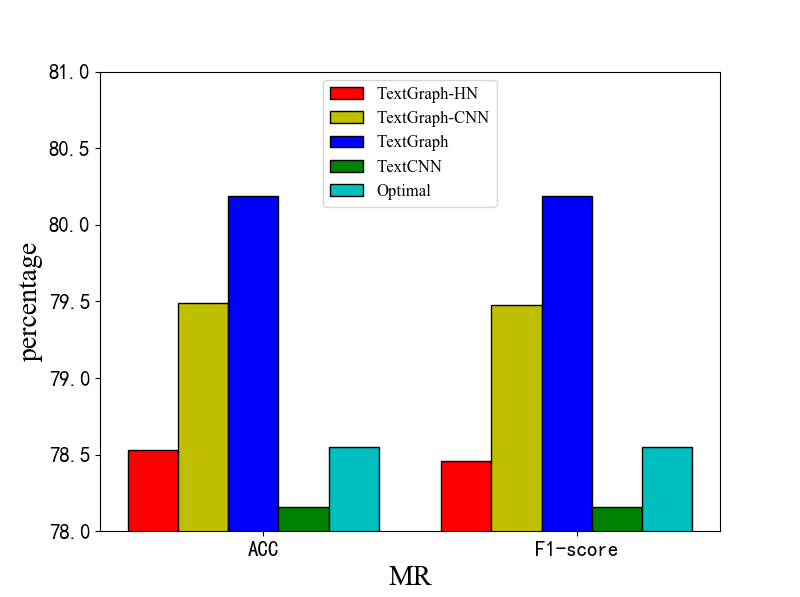
\includegraphics[width=1\textwidth]{pic/HisMR.png}
    \caption{MR数据集ACC和F1-score}
    \label{MR_acc_f1}
    \end{minipage}
    \quad
    \begin{minipage}[t]{0.5\linewidth}
    \centering
    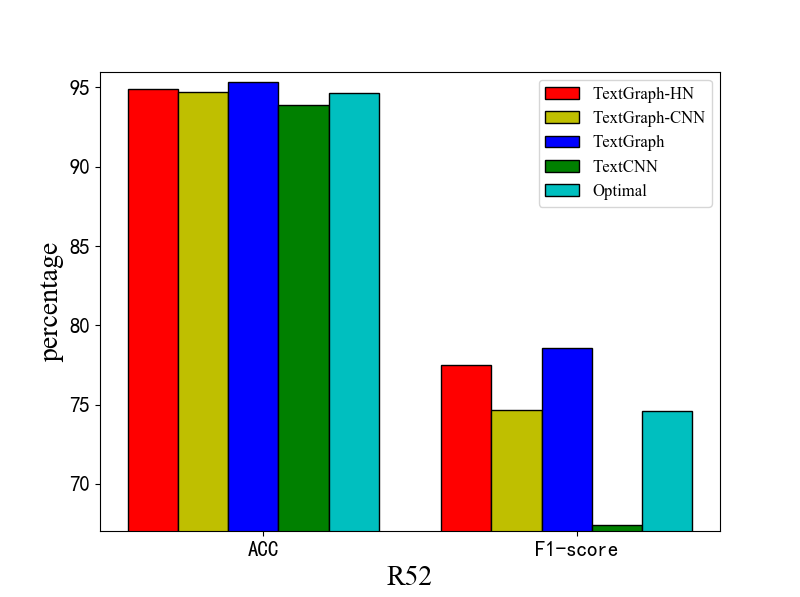
\includegraphics[width=1\textwidth]{pic/HisR52.png}
    \caption{R52数据集ACC和F1-score}
    \label{R52_acc_f1}
    \end{minipage}
\end{figure*}

\begin{figure*}[htb]
    \begin{minipage}[t]{0.5\linewidth}
    \centering
    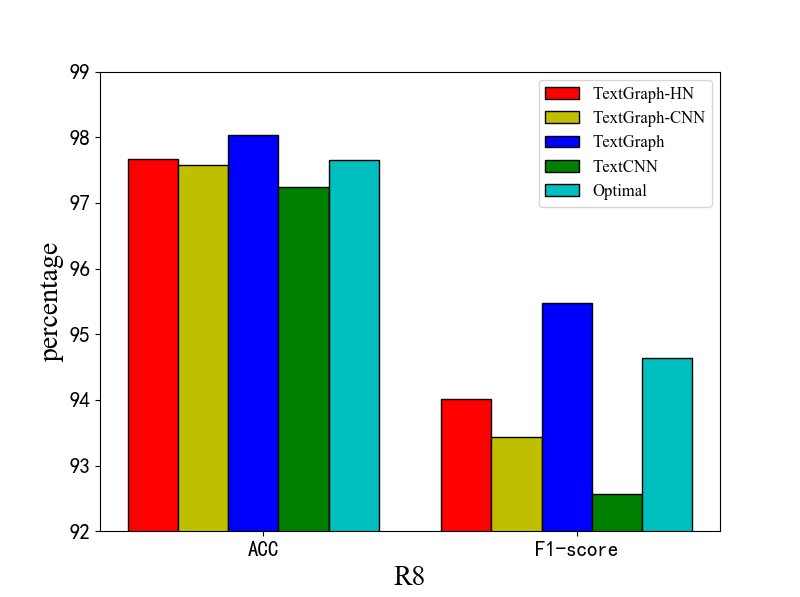
\includegraphics[width=1\textwidth]{pic/HisR8.png}
    \caption{R8数据集ACC和F1-score}
    \label{R8_acc_f1}
    \end{minipage}
    \quad
    \begin{minipage}[t]{0.5\linewidth}
    \centering
    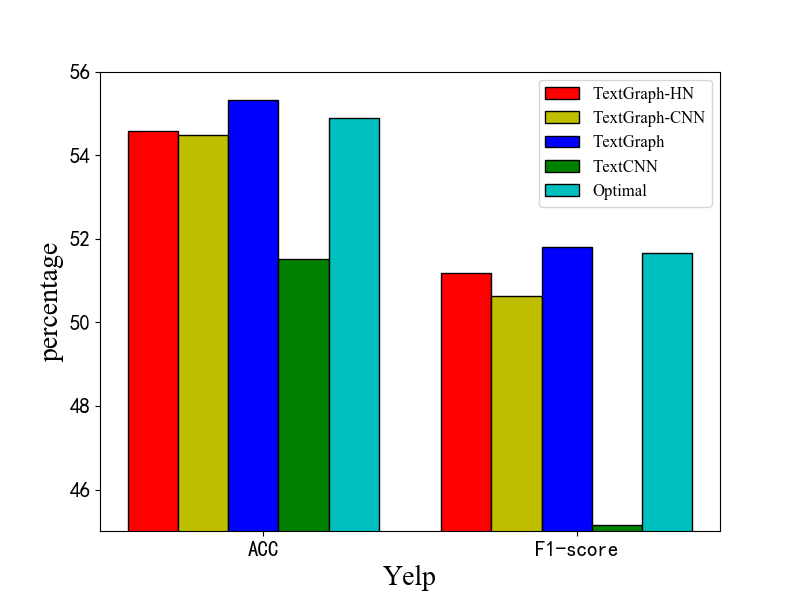
\includegraphics[width=1\textwidth]{pic/HisYelp.png}
    \caption{Yelp数据集ACC和F1-score}
    \label{Yelp_acc_f1}
    \end{minipage}
\end{figure*}

\subsection{训练集比例的影响}
为了了解训练集大小对模型文本分类性能的影响,本章从R8的训练集中随机选取了2.5\%、5\%、7.5\%、10\%、12.5\%等不同百分比的样本作为
训练集,其他的均作为测试集来评价训练模型分类性能。如图\ref{R8_acc}和图\ref{R8_f1-score}所示,展示了不同比例下的模型分类准确率和F1分数。
从图上可以看出,TextGraph即使在低比率的情况下依然高于所有对比方法。TextGraph在训练样本数为2.5\%的情况下获得91.9\%的准确率,
而大多数基线的准确率低于85\%,仅有同样采用了GCN模型的textGCN与本章提出的方法差距不大。此外,TextGraph的$F1$得分为74.71\%,而TextCNN的得分为36.82\%。
这些结果表明,与textGCN采用了语料库中的信息类似,TextGraph的文本图中的超节点能够捕获全局信息,以及语料库中的潜在信息——主要是通过
TF-IDF得到的,另一方面文本图的构造方式能够很好地反映短文本的结构,可以作为一些人为定义的潜在知识。这些信息的结合,使得模型在低比例训练集情况下依然
能够展现较为良好的性能。

\begin{figure*}[htb]
    \begin{minipage}[t]{0.5\linewidth}
    \centering
    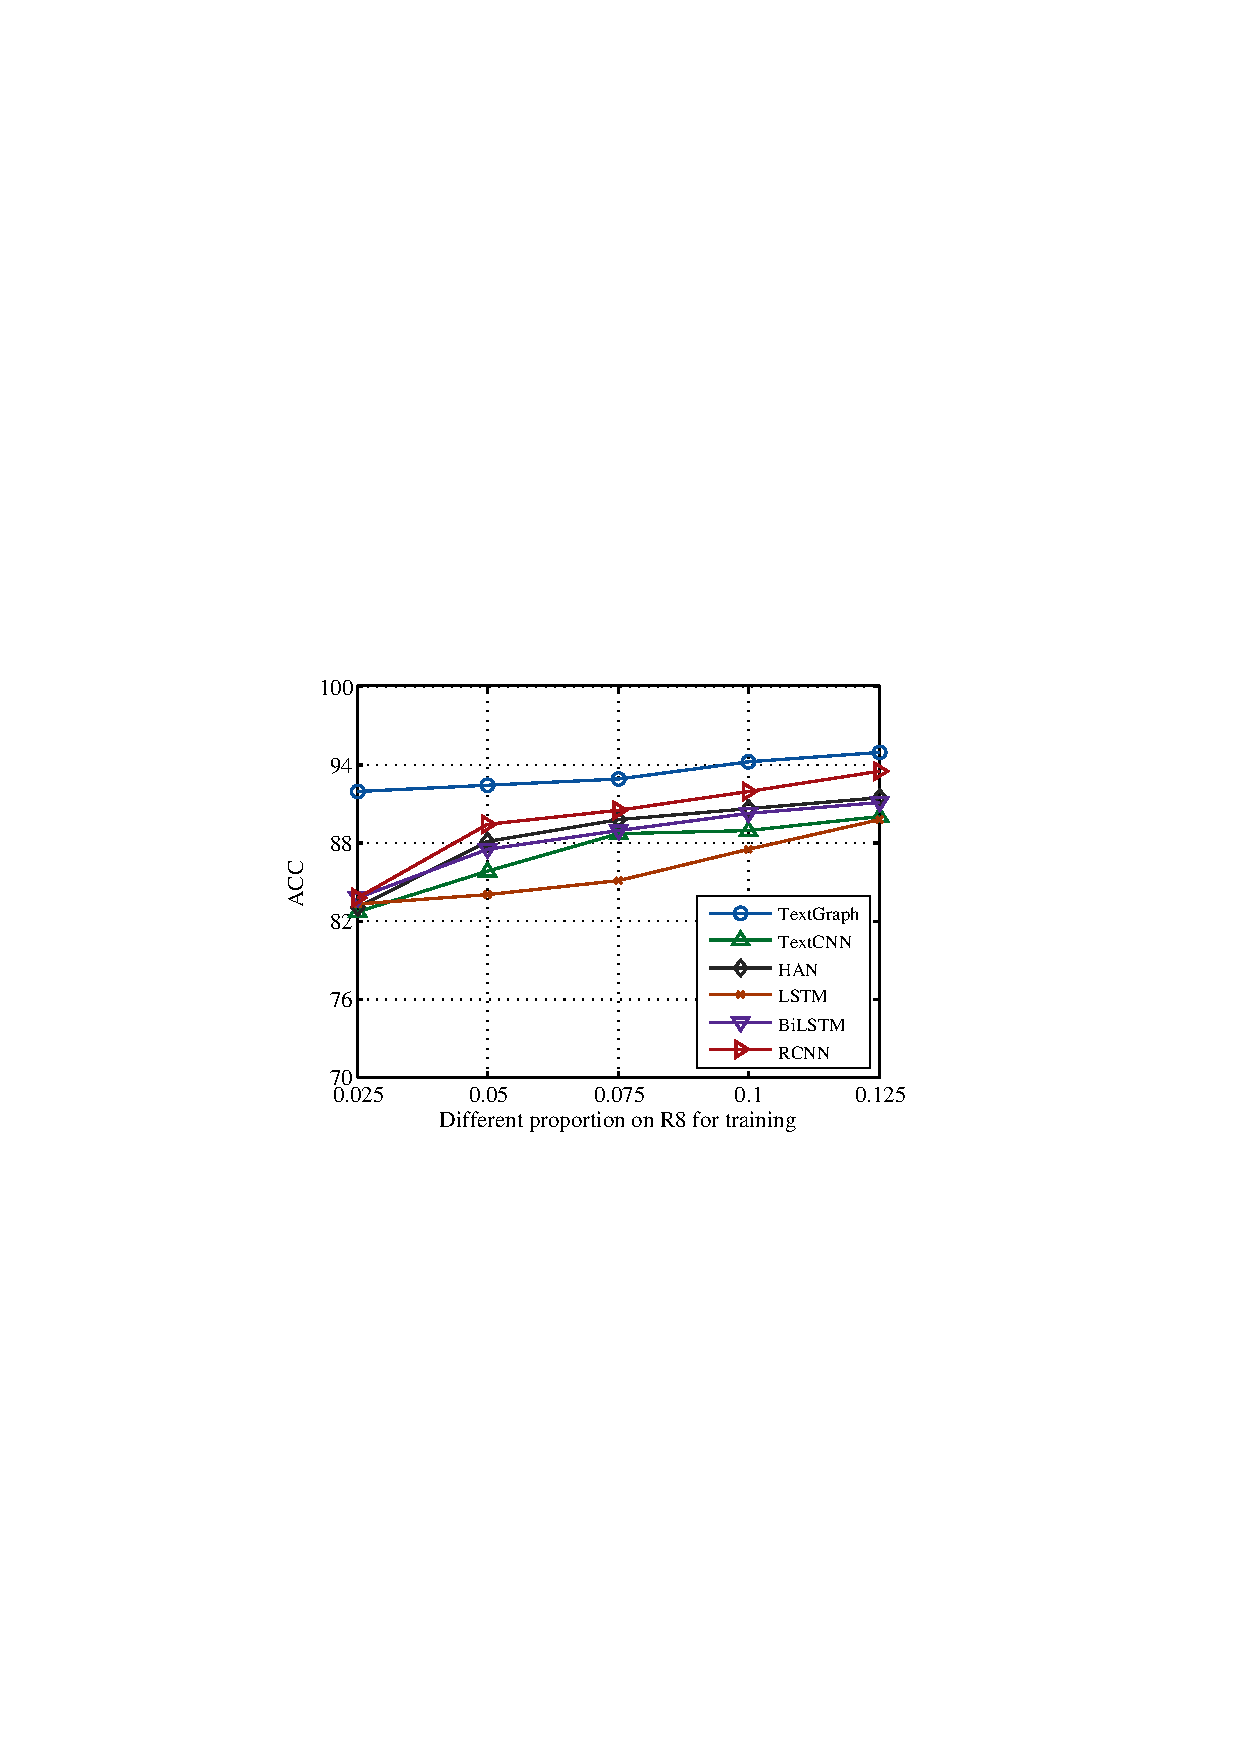
\includegraphics[width=1\textwidth]{pic/R8_acc.pdf}
    \caption{不同比例训练集分类ACC}
    \label{R8_acc}
    \end{minipage}
    \quad
    \begin{minipage}[t]{0.5\linewidth}
    \centering
    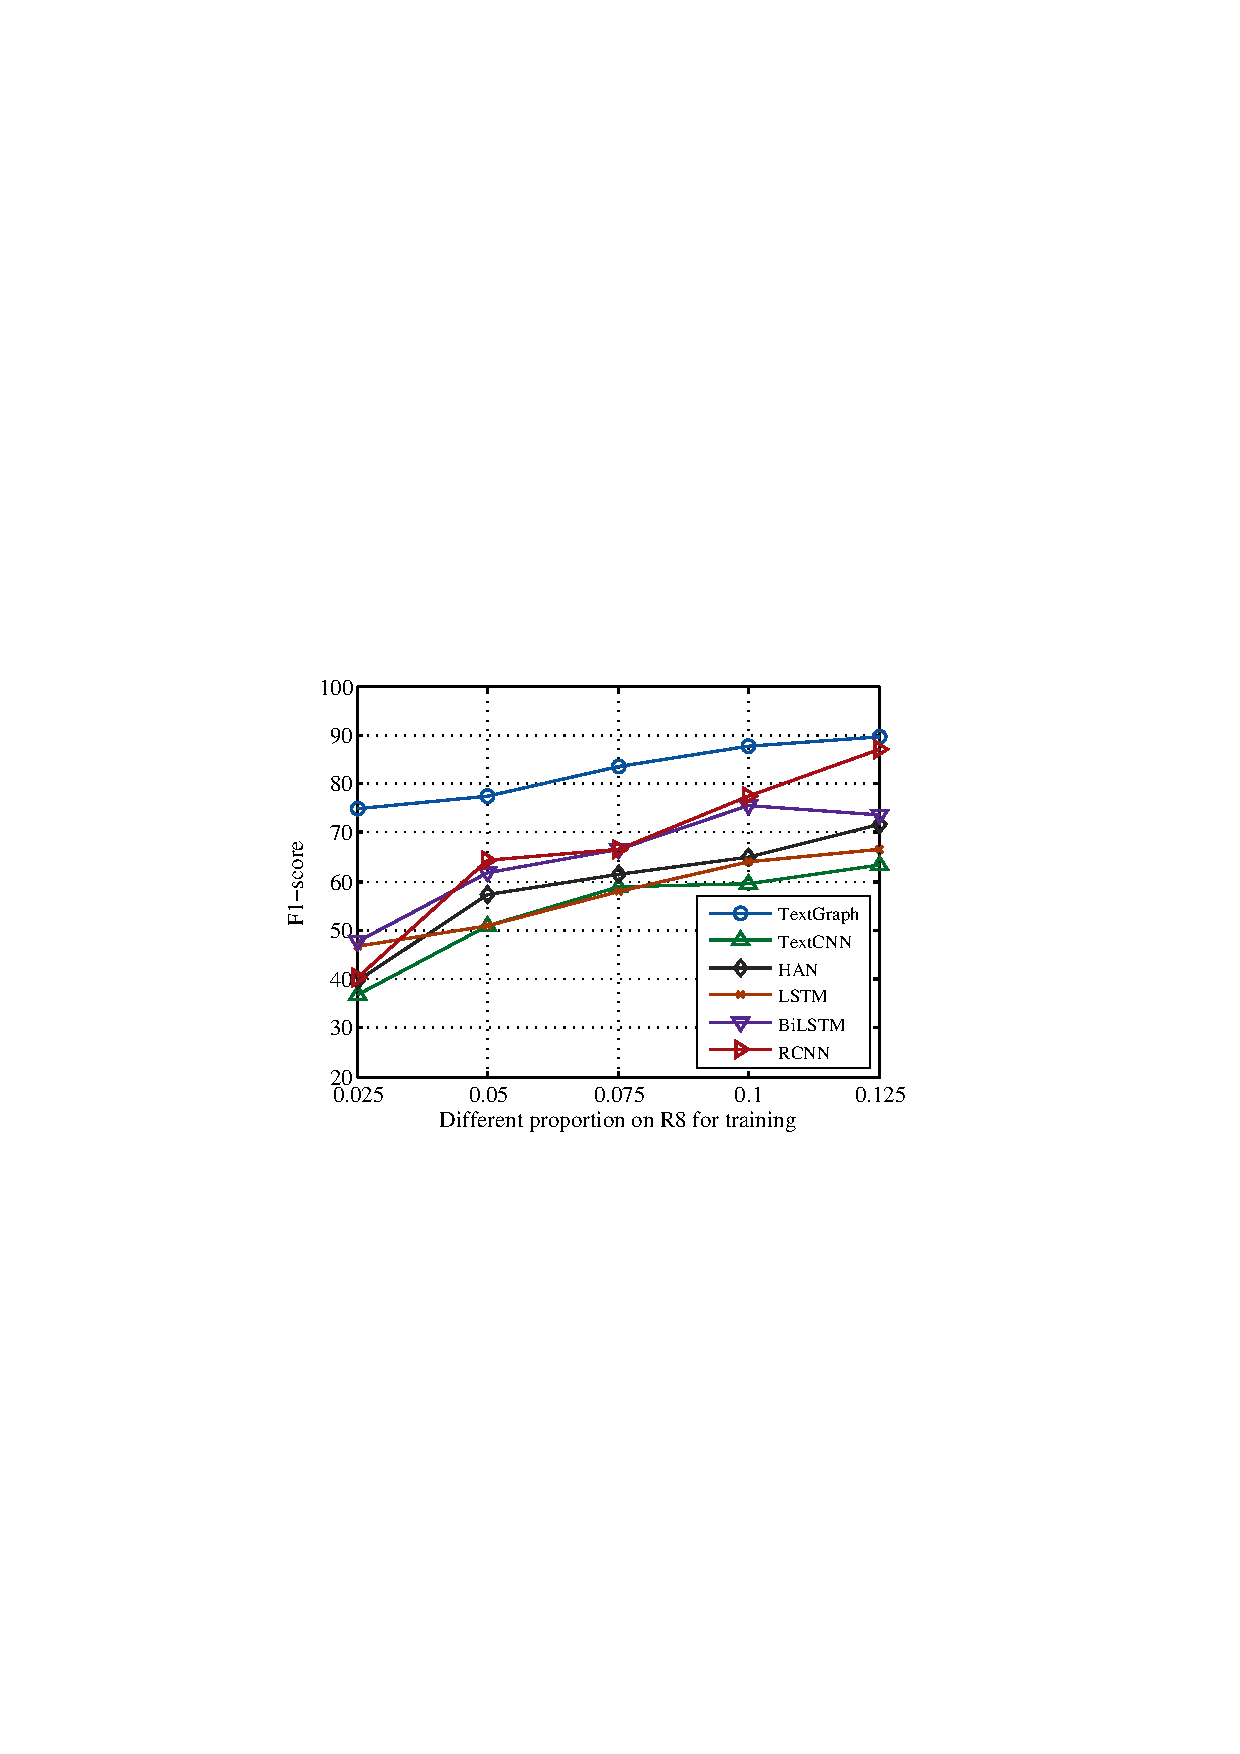
\includegraphics[width=1\textwidth]{pic/R8_f1-score.pdf}
    \caption{不同比例训练集分类F1-score}
    \label{R8_f1-score}
    \end{minipage}
\end{figure*}

\subsection{文本向量可视化分析}
为了更好的理解TextGraph的分类性能,本章采用基于t-SNE的方法将不同模型生成的文本向量压缩至二维平面进行可视化观察。
如图\ref{r8_embeding}所示,展示了采用LSTM模型进行训练的R8数据集的文本向量,该实验室采用5\%的比例训练集进行训练,
然后对测试集上的数据进行可视化分析。图中的每一个点代表了一个文本向量压缩后的向量表示。相同的颜色代表这个文本属于
同一个分类标签。从图中可以看出即使是同一类的样本,也未能完全聚集在一起,且明显成“条状”,与其他类型的样本交错在一起。
在同一个类别簇下,也杂含了许多其他类别的样本,界限并不分明。如图\ref{R8_TextGraph}所示,展示了采用TextGraph模型经过
同样比例训练集训练后的测试文本向量。相比于LSTM的方法,该模型生成的同一类别的向量表示更加紧凑,不同类别之间的界限更具分明。
如LSTM模型生成的样本中,蓝色和橘色样本交织在一起,这样对于分类来说难以区分它们,而本章提出的模型,这两种类别区分明显
仅有少量的样本交错,这样便有较高的区分度,使得模型分类准确率更高。

\begin{figure*}[htb]
    \begin{minipage}[t]{0.5\linewidth}
    \centering
    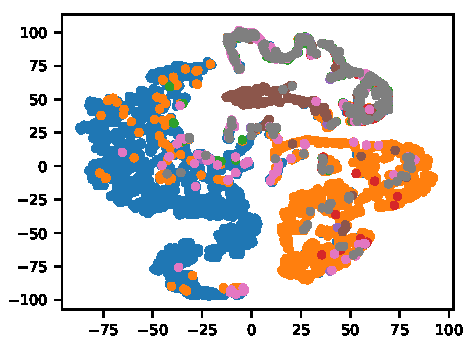
\includegraphics[width=1\textwidth]{pic/R8-RNN.pdf}
    \caption{LSTM模型的R8文本数据集可视化}
    \label{r8_embeding}
    \end{minipage}
    \quad
    \begin{minipage}[t]{0.5\linewidth}
    \centering
    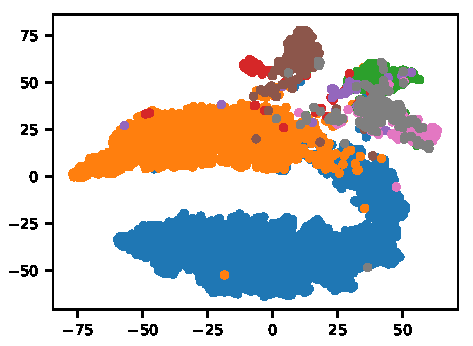
\includegraphics[width=1\textwidth]{pic/R8-TextGraph.pdf}
    \caption{TextGraph模型的R8文本数据集可视化}
    \label{R8_TextGraph}
    \end{minipage}
\end{figure*}

\section{本章小结}
本章提出了一个基于图网络的文本分类模型,为序列相关的研究提供了一点另类的思路。方法首先对文本进行建模,对每一文本根据单词之间的先后顺序
构建了一个独立的图结构。同时采用语料库中单词与文本的关联构建了一个连接文本中所有单词的超节点,用以
捕获文本的全局信息以及语料库中的部分关联信息。将构建好的图输入到GCN网络中学习,这些步骤的实现都能促进模型学到
更好的单词表示。之后再采用CNN模型对新的单词向量进行局部信息以及关键信息的捕捉。与其他常用的模型相比,本章提出的方法在
准确率和F1分数上均有提升。同时在低比例训练集的情况下也能展现良好的性能。